\subsection{Kullback-Leibler (KL) divergence}
\label{appendix:kl_divergence}

\begin{figure}
    \centering
    \caption{Showcase of KL-Divergence of three different normal distributions. The divergence between two normal distributions can occur in both mean and variance. Mean (or expectation) is the center of the distribution, while variance is the spread of the distribution.}
    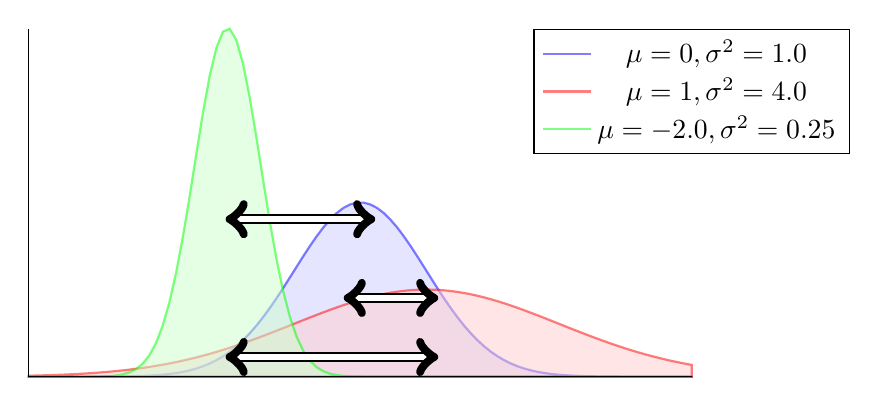
\begin{tikzpicture}
        \begin{axis} [
          no markers, 
          domain=-5:5, 
          samples=100,
          axis lines*=left, 
          height=6cm, 
          width=10cm,
          xtick=\empty, 
          ytick=\empty,
          enlargelimits=false, 
          clip=false, 
          axis on top,
          grid = major,
          legend style={at={(1,1)}, anchor=north, legend columns=1},
        ]

        % Define variables (mean, variance)
        \pgfmathsetmacro{\muA}{0}
        \pgfmathsetmacro{\sigmaA}{1}
        \pgfmathsetmacro{\varA}{\sigmaA^2}
        
        \pgfmathsetmacro{\muB}{1}
        \pgfmathsetmacro{\sigmaB}{2}
        \pgfmathsetmacro{\varB}{\sigmaB^2}
        
        \pgfmathsetmacro{\muC}{-2}
        \pgfmathsetmacro{\sigmaC}{0.5}
        \pgfmathsetmacro{\varC}{\sigmaC^2}
    
        % Blue
        \addplot[blue, thick, fill=blue!20, opacity=0.5] 
        {1/sqrt(2*pi*\sigmaA^2) * exp(-0.5 * ((x-\muA)/\sigmaA)^2)} \closedcycle;
        \addlegendentry{$\mu = \muA, \sigma^2 = \varA$};

        % Red
        \addplot[red, thick, fill=red!20, opacity=0.5] 
        {1/sqrt(2*pi*\sigmaB^2) * exp(-0.5 * ((x-\muB)/\sigmaB)^2)} \closedcycle;
        \addlegendentry{$\mu = \muB, \sigma^2 = \varB$};

        % Green
        \addplot[green, thick, fill=green!20, opacity=0.5] 
        {1/sqrt(2*pi*\sigmaC^2) * exp(-0.5 * ((x-\muC)/\sigmaC)^2)} \closedcycle;
        \addlegendentry{$\mu = \muC, \sigma^2 = \varC$};
        
        \end{axis}

        % Arrows between distributions
        % Blue, Green
        \draw[{<._[sep=-4pt]}-{_[sep=-4pt].>}, line width=0.8pt, double, double distance=2pt] (2.5,2) -- (4.4,2);
        % Green, Red
        \draw[{<._[sep=-4pt]}-{_[sep=-4pt].>}, line width=0.8pt, double, double distance=2pt] (2.5,0.25) -- (5.2,0.25);
        % Blue, Red
        \draw[{<._[sep=-4pt]}-{_[sep=-4pt].>}, line width=0.8pt, double, double distance=2pt] (4,1) -- (5.2,1);

    \end{tikzpicture}
    \label{fig:kl_divergence}
\end{figure}

Kullback-Leibler (KL) divergence allows us to measure the difference between two probability distributions, $P$ and $Q$. It essentially quantifies how much information is lost when using distribution $Q$ to approximate distribution $P$.

In various applications, we deal with situations where we have a true underlying distribution (P) representing the actual data generation process, but we might not know its exact form. We might have another distribution (Q), perhaps a model we've built, that we want to use to represent or approximate the true distribution. KL divergence helps us understand how well Q captures the information present in P. In other words, \textbf{how much diverged the distribution Q is from the distribution P}. See figure \ref{fig:kl_divergence} for a visual representation.

The mathematical formula for KL-divergence is:

\begin{equation}
\label{eq:kl-divergence}
    D_{KL}(P || Q) = \sum_{x \in X} P(x) \cdot log(\frac{P(x)}{Q(x)})
\end{equation}

where $x \in X$ represents all the possible values within the data space ($X$).

A KL-divergence value of 0 indicate that the distribution $Q$ perfectly captures the distribution $P$, and larger numbers indicate higher disparity.

KL-divergence measures information lost, so if both $P,Q$ are Gaussian distributions with the same mean and standard deviation, we have no information lost. But if the standard deviation or the mean is different, KL-divergence measures that. On the other hand, directly integrating the distributions and measuring the area under the curve (AUC) will not show information loss if the standard deviation is the same, but the mean is different.


Other notations are used as well: $p_\theta(x_i), q_\phi(x_i)$. Most of the time we are dealing with small numbers in the probabilities, which will get multiplied with other small numbers, which may result in rounding to zero. So instead we generally compute \textbf{log-likelihood}: $log\ p_\theta(x_i), log\ q_\phi(x_i)$. Now to compare two distributions we can compute the difference: $log\ p_\theta(x_i) - log\ q_\phi(x_i)$ and if that subtraction result in zero that means that our approximated distribution $q$ is identical to ground truth $p$. We can rewrite it like so: 

\begin{equation}
\label{eq:log-likelihood}
    log\ [\frac{p_\theta(x_i)}{q_\phi(x_i)}]
\end{equation}

which is also sometimes called \textbf{log-likelihood ratio}.

In reality we are only interested in the \textbf{average difference} between $p_\theta$ and $q_\phi$. Because we are dealing with random variables $x \in X$, instead of average we say \textbf{expected value} of a random variable. Weighted average of instances of random variables is:

\begin{equation*}
    \mathbb{E}_{p_\theta} [X] = \sum_{i=1}^{\infty} x_i p_\theta(x_i)
\end{equation*}

where $x_i$ is the state of the random variable, and $p_\theta(x_i)$ is the weight (weight of contribution to the average). A more general formulation is given by:

\begin{equation*}
    \mathbb{E}_{p_\theta} [h(X)] = \sum_{i=1}^{\infty} h(x_i) p_\theta(x_i)
\end{equation*}

where $h(X), h(x_i)$ is a function of random variable $x_i \in X$. This formulation works for discrete random variable, here is the formulation for continuous random variable:

\begin{equation*}
    \mathbb{E}_{p_\theta} [h(X)] = \int_{\mathbb{R}} h(x) p_\theta(x) dx
\end{equation*}

Lets get back to the average likelihood (equation \ref{eq:log-likelihood}), we can set $h(X) = log\ [\frac{p_\theta(x_i)}{q_\phi(x_i)}]$ and we get:

\begin{equation*}
    \sum_{i=1}^{\infty} p_\theta(x_i) log\ [\frac{p_\theta(x_i)}{q_\phi(x_i)}]
\end{equation*}

where $p_\theta(x_i)$ is the weight. This equation is called the \textbf{KL-divergence}:

\begin{equation}
\label{eq:kl_divergence}
    \mathbb{E}_p [log\ \frac{p_\theta(x_i)}{q_\phi(x_i)}]
    =
    \sum_{i=1}^{\infty} p_\theta(x_i) log\ [\frac{p_\theta(x_i)}{q_\phi(x_i)}]
    =
    D_{KL} (p_\theta || q_\phi)
\end{equation}

In short, this is the expected value of the log-likelihood ratio (of discrete random variable). For continuous random variable we get similar formula:

\begin{equation}
\label{eq:kl_divergence_continous}
    \mathbb{E}_p [log\ \frac{p_\theta(x_i)}{q_\phi(x_i)}]
    =
    \int_{\mathbb{R}} p_\theta(x) log\ [\frac{p_\theta(x)}{q_\phi(x)}] dx
    =
    D_{KL} (p_\theta || q_\phi)
\end{equation}

One problem we are dealing with is the infinity space in both equations.  To get around it we can use the \textbf{law of large numbers} which says:

\begin{equation*}
    \frac{1}{N} \sum_{i=1}^N h(x_i) \approx \mathbb{E}_p [h(X)]
\end{equation*}

and we get:

\begin{equation}
    D_{KL} (p_\theta || q_\phi) \approx
    \frac{1}{N} \sum_{i=1}^N log\ [\frac{p_\theta(x_i)}{q_\phi(x_i)}]
\end{equation}

Credit to \cite{dk-divergence-math-explanation} for the math explanation.